\section{What is artificial intelligence?}
\setauthor{Romeo Bhuiyan}
The concept of AI has a long history that dates back to ancient times,
when people first tried to build machines that could mimic human abilities.
In the modern era, the term \textit{AI}  was first coined in 1956 by computer scientist 
John McCarthy, who defined it as \textit{the science and engineering of making 
intelligent machines} \footnote{johnmcCarthy:1956}.
% \cite[the science and engineering of making intelligent machines]{johnmcCarthy:1956} .

Today, these machines are designed to be able to perform tasks that typically 
require human intelligence, such as visual perception, speech recognition,
decision-making, and understanding natural language. AI can be applied to a wide
range of fields, from healthcare and finance to education and transportation,
with the goal of making systems more efficient and effective.
AI can be classified into two broad categories: \textit{narrow or weak AI},
which is designed to perform a specific task, and \textit{general or strong AI},
 which has the ability to perform any intellectual task that a human being can perform. \cite{KindsOfAI}

\section{Philosophy of artificial intelligence}
\setauthor{Christoph Lasinger}
Can a machine think? Thinking seems to be one of, if not the most important part of being human, as seen in René Descartes' 
first principle of philosophy “Cogito, ergo sum” (“I think, therefore I am”). So it goes to reason that, if we, as 
homo sapiens, were to see us superior to other animals on earth, it would be our intelligence, our conscious thinking, 
that would seem to differentiate us, make us special. Assuming this line of reasoning to be true, then it would only 
seem logical to think that we, as humans, are superior to machines in that regard as well. But what if that were to be taken away?

Throughout the course of history humans have practically been obsessed with self-imitation, be it wall-paintings, 
statues, portraits, photos, films or today's machines. The earliest example of artificial humans may be Greek gods, 
or rather Greek mythology as a whole, including for example architect and craftsman Daedalus, who created statues and 
machines that were sometimes impossible to distinguish from real human beings. Ancient Egypt also featured statues of 
gods behaving like humans and even though they were being controlled not by a god, but through complex mechanisms, 
such as quicksilver or hydraulics, or even simple puppeteering strings, the Egyptians still feared and revered them. 
They saw it not as blasphemy but as gods acting through guided souls, even though they might be that of a master and puppet.

However, not everyone would view such creations as positive as the Greeks and Egyptians. As even before their 
time a different culture, or to be more accurate religion had rules regarding artificial humans, the so called 
ten commandments, of which the second one states “You shall not make for yourself a carved image, or any likeness 
of anything that is in heaven above, or that is in the earth beneath, or that is in the water under the earth. 
You shall not bow down to them or serve them, for I the Lord your God am a jealous God ...". Of course, any religious 
text is open to interpretation, but it seems a rather popular one was that of Hermes Trismegistor, purported author 
of the Hermetica, a series of ancient texts that lay the basis of philosophical systems known as Hermetecicism, 
who stated that man has created statues, infused with the souls of demons and angels through holy rituals.

The purpose of mentioning these two views regarding artificial humans is that they are essentially the 
two fundamental views of the western world regarding “thinking machines”, or artificial intelligence, 
as well. This can be seen in statements made by both critics and proponents of AI. \cite{Denkmaschinen}
\newpage
\section{The future of artificial intelligence}
\setauthor{Romeo Bhuiyan}
The future of AI is difficult to predict with certainty,
but it is likely that AI will continue to advance and become 
increasingly integrated into our daily lives. AI has the potential 
to revolutionize many industries, from healthcare and transportation 
to education and finance. It could also have a major impact on the job 
market, with some jobs being automated by AI and other jobs being created 
to support the technology. However, it is important to consider the potential 
drawbacks of AI and ensure that it is developed and used ethically. Overall, 
the future of AI seems promising, but it is important to approach it with caution 
and consideration. As the future of AI is very likely to lie somewhere between a very 
positive one (extreme optimism) and a very negative one (extreme pessimism), it makes sense 
to analyze those two specifically.

An extremely pessimistic future of AI in the world would involve the 
technology being used in ways that are harmful to humanity. In this scenario, 
AI could be used to create weapons of mass destruction, or to control and manipulate 
people for nefarious purposes. It could also be used to create a surveillance state, 
where people's every move is monitored and tracked. Additionally, the widespread use of 
AI could lead to widespread job loss and economic instability, as many jobs are automated 
and replaced by machines. In a worst-case scenario, the development of AI could even lead 
to a global conflict over control of the technology.

An extremely optimistic future would entail an AI with highly advanced and 
integrated technology that is able to solve many of the world's most pressing 
problems. In this scenario, AI would be used to improve healthcare, reduce poverty 
and inequality, and address climate change. It would also be used to make transportation 
faster, safer, and more efficient, and to improve education by providing personalized learning 
experiences for students. Moreover, AI could be used to help us better understand and protect the 
natural world, and to explore the universe. Overall, this extremely optimistic future of AI would 
involve the technology being used to enhance and improve human life in countless ways.



\section{The functional concept of neural networks}
\setauthor{Romeo Bhuiyan}
A neural network is a type of machine learning algorithm modeled 
after the structure and function of a human brain (neural linking). 
It is composed of many interconnected processing nodes, called neurons, 
which work together to process information. 
\\
\begin{figure}[htb]
    \centering
    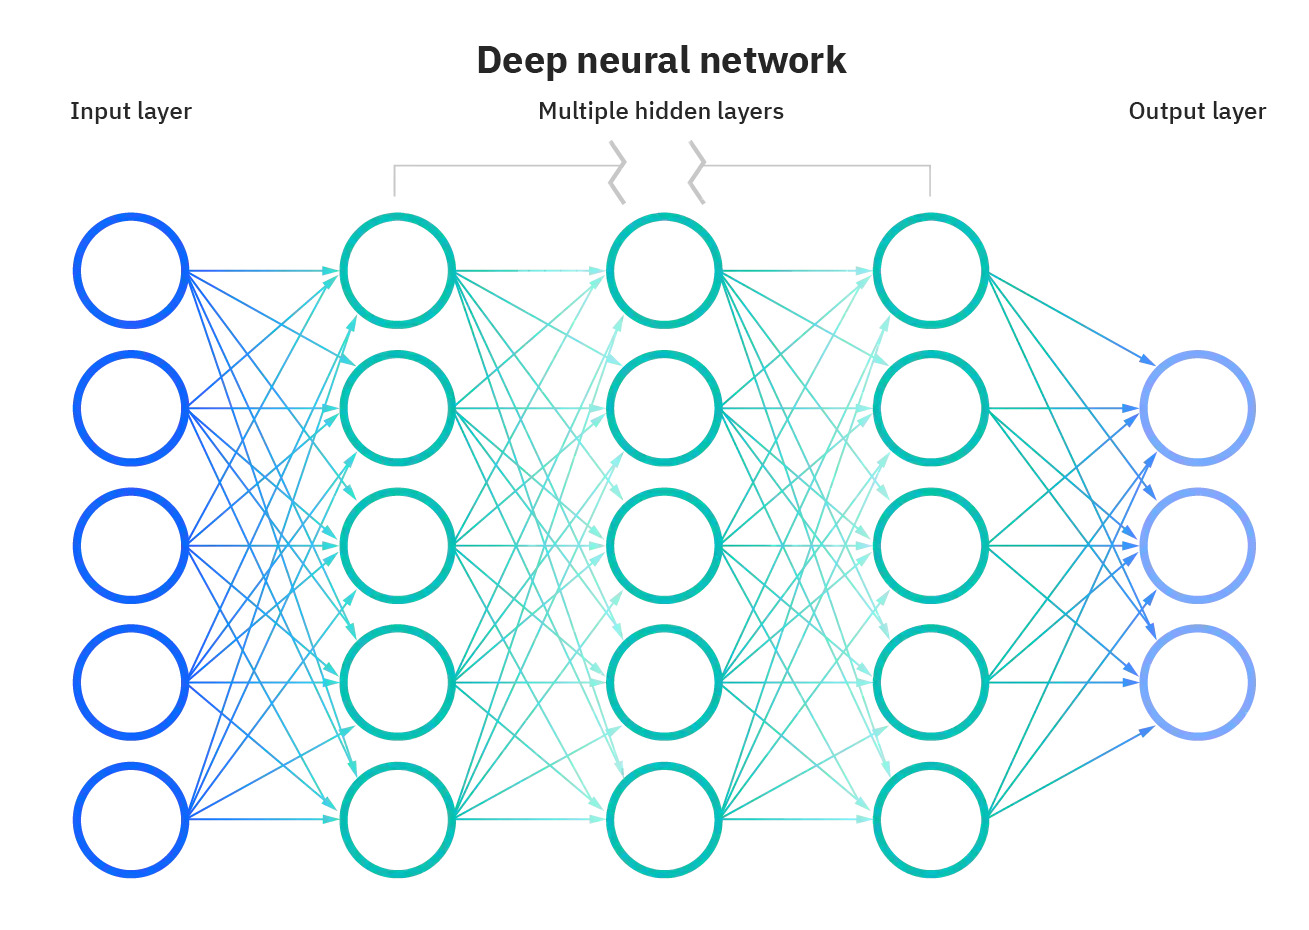
\includegraphics[width=0.8\textwidth]{pics/neuralnetwork.jpg}
    \caption{Complex neural network}
    \label{fig:neuralnetwork}
    \cite{IBM}
\end{figure}
\\
As shown in figure \ref{fig:neuralnetwork}, each neuron receives input from other neurons, processes that information, 
and produces an output. This output is then passed on to other neurons in the next 
layer of the network. In this way, information is passed through the network, from the 
input layer to the output layer, allowing the neural network to learn and make predictions
based on the data it is given. \cite{book1}

The specific details of how a neural network works can vary depending on its architecture
and the type of problem it is being used to solve. But in general, a neural network is able 
to learn from data by adjusting the strength of the connections between its neurons, these 
connections being called weights, based on the input it receives. Over time, the network is 
able to improve its predictions by adjusting these weights in a way that minimizes errors 
between the network's output and the correct output.

\subsection{Solving methods}
There are three basic methods for solving problems: 
search-, knowledge-, and algorithmic methods. 
Every method involves searching through a space of possible
solutions whilst optimizing a pre-defined evaluation function, 
that can lead to the following \emph{Combinatorial explosion} as shown below in the figure \ref{fig:combiexplo}. 
The methods can range from \emph{simplex hill climbing via alpha-beta pruning techniques} to \emph{knowledge chunking}. 

\textbf{Simplex hill climbing via alpha-beta pruning techniques} is a combination of two different methods used to solve optimization problems 
in artificial intelligence. Simplex hill climbing is an iterative method that tries to find the maximum or minimum value of an objective function 
by repeatedly changing the input values and evaluating the function at each point until a peak or valley is found. The alpha-beta pruning 
technique is a search algorithm used in game theory to reduce the number of nodes evaluated in a minimax algorithm.

The simplex hill climbing algorithm starts with a randomly selected point in the search space and then moves to the neighboring points 
in each iteration, depending on the function's value at that point. The goal is to eventually reach the point that maximizes or minimizes 
the function, depending on the problem's objective. However, this method can be slow, especially for higher-dimensional search spaces, 
as the search may get stuck in a local maximum or minimum that is not the global optimum.

To speed up the search process, the alpha-beta pruning technique can be applied. This technique uses a cutoff mechanism to eliminate 
parts of the search tree that cannot influence the final result. By pruning the tree, the search algorithm can avoid evaluating nodes 
that are unlikely to lead to a better solution, reducing the number of evaluations required to find the optimal solution. This approach 
is particularly useful for search spaces with many branches, such as game trees.

By combining these two techniques, simplex hill climbing via alpha-beta pruning can efficiently and effectively search for optimal 
solutions in complex optimization problems. The algorithm is particularly useful for problems that have large search spaces or are 
difficult to solve with other methods. However, like any algorithm, it has its limitations and may not always be the best choice 
for every problem. \cite{pruning}

\textbf{Knowledge chunking} is a technique used in artificial intelligence to improve problem-solving efficiency by breaking down complex problems 
into smaller, more manageable parts or \emph{chunks}. The process of chunking involves identifying patterns and relationships within a problem 
and grouping similar elements together into chunks. These chunks are then treated as separate entities, allowing for more efficient processing and retrieval from memory.

This has been shown to be effective in a range of AI applications, including natural language processing, expert systems, 
and machine learning. By breaking down complex problems into smaller, more manageable pieces, knowledge chunking allows AI systems to 
more effectively reason, learn, and make decisions. Additionally, the use of chunking can improve the scalability and generalizability 
of AI systems by allowing them to better handle larger, more complex datasets. Overall, knowledge chunking is a valuable technique for 
improving the efficiency and effectiveness of AI systems across a range of applications. \cite{knowledgechunking}

Example: the chess endgame of king and three pawns versus king 
and three pawns requires an explicit table of half a billion 
moves and a run-time of ten quadrillion years to evaluate all
possibilities. The success of the CMU \emph{chunker} program which
uses chess domain knowledge chunks is that it reduces this
run-time to about one minute.
\\
\begin{figure}[htb]
    \centering
    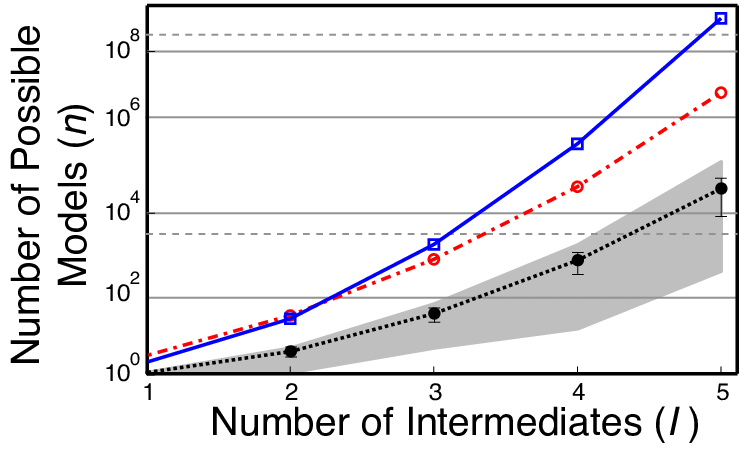
\includegraphics[width=0.5\textwidth]{pics/combiexplo.png}
    \caption{Combinatorial explosion} 
    \cite{combiexplo}
    \label{fig:combiexplo}
\end{figure}
\\
\section{Explanation of face tracking}
\setauthor{Romeo Bhuiyan}
Face tracking is a technology that allows a computer or device to identify
and monitor the movements of a person's face in real time. 
This is typically done using a combination of computer vision 
algorithms and specialized hardware, such as a camera or depth sensor. \cite{book2}

To track a face, the system first detects the face in 
the video feed from the camera or depth sensor. This is 
typically done using a machine learning algorithm trained to 
recognize faces in images. Once the face has been detected, 
the system then uses various techniques to track the movements 
of the face, such as tracking the position of key facial features
(like eyes and mouth) over time, as seen below in figure \ref{fig:facetracking}.
 This allows the system to accurately follow the face as it moves within the frame, even if it 
turns or changes orientation.

The resulting data can be used for a variety of 
purposes, such as enabling facial recognition 
(to identify who the person is), animating virtual characters, 
or controlling a user interface.
\\
\begin{figure}[htb]
    \centering
    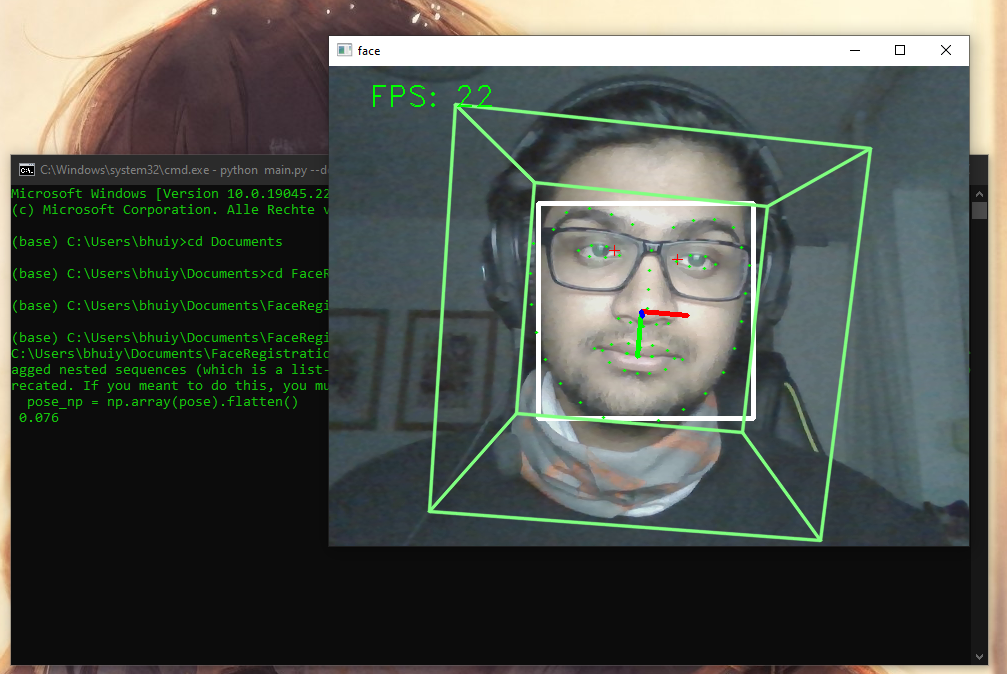
\includegraphics[width=0.8\textwidth]{pics/bhuiyanfracetracking.png}
    \caption{Face tracking experiment done by Romeo Bhuiyan}
    \label{fig:facetracking}
\end{figure}
\\
\section{Explanation of body tracking}
\setauthor{Romeo Bhuiyan}
Body tracking is the process of using technology to track the movement of a person's body.
This is typically done using sensors or cameras that capture the movement of the body and 
then use algorithms to interpret that movement and translate it into digital data that can 
be used for various purposes. 

To track a body, the algorithm first detects the presence of a body in the video or data.
It then uses various techniques to identify specific features of the body, such as the limbs, 
torso, or other distinctive features. This allows the algorithm to track the body as it moves over time. 

In addition to tracking the location of the body, some algorithms can also track 
other features, such as body movements or gestures. This allows them to be used for a 
variety of applications, such as video surveillance, virtual reality, gaming, human-computer 
interaction, and fitness tracking.

\section{Comparison of machine learning frameworks}
\setauthor{Romeo Bhuiyan}
In this case face tracking was needed in order to get a virtual model animated. 
The two libraries MediaPipe and TensorFlow.js were tested using python to decide 
which one is better suited for our purpose. It is difficult to say which approach 
is more suitable for face, hand, and body tracking in the browser, as it will depend 
on the specific requirements and constraints of one's project. Both MediaPipe and 
TensorFlow.js are powerful tools that can be used to perform these tracking tasks, 
but they have different strengths and limitations.

\textbf{MediaPipe} is a library developed by Google that is specifically designed 
for real-time multimedia processing tasks, such as hand and face tracking. 
It is written in C++ with some Python bindings and can be used to build cross-platform 
pipelines for performing various computer vision and machine learning tasks. MediaPipe is 
optimized for low-latency, real-time processing and is used to build applications that run 
on a variety of platforms, including the browser. \cite{Mediapipe}

In contrast, \textbf{TensorFlow.js} is a JavaScript library for training and deploying machine 
learning models in the browser. It is based on the TensorFlow library, a popular machine 
learning library developed by Google. TensorFlow.js allows you to build and train machine 
learning models using JavaScript, and it can be used to perform a variety of tasks, including 
image and text classification, time series forecasting, and natural language processing. \cite{Tensorflow}

In \textbf{Conclusion}, both MediaPipe and TensorFlow.js are able to handle face and hand
tracking in the browser, but personal experiments were conducted based on connectivity with the VRM model rigging in order to find out 
that they have different trade-offs and may be better suited
for different types of projects. MediaPipe is optimized for real-time processing and is
good for building applications that require low latency, such as augmented reality or
interactive applications. However, TensorFlow.js is a general-purpose machine learning
library that is suited for building machine learning models and deploying them in the
browser, but it may not be as efficient for real-time processing as MediaPipe. 
At the end of the Python experiment, the camera controls worked better with only one of these libraries, 
and thinking that more content will likely be added to the project in the future, we have decided 
to use MediaPipe as our real-time multimedia library solution.

\section{Optimizing artificial intelligence models through training}
\setauthor{Romeo Bhuiyan}
AI training is a crucial process in the development of AI systems. 
It involves feeding large amounts of data into an AI model to enable it to learn and perform 
tasks accurately. The quality of the training data and the algorithms used to train the model 
determine the effectiveness of the AI system.
The importance of AI training lies in its ability to provide a platform for creating smarter 
and more capable AI systems that can perform complex tasks with a high degree of accuracy. 
It allows AI systems to make predictions, process vast amounts of data, and automate tasks, 
making them more efficient and effective.
For example, AI training is used in natural language processing to teach AI models how to 
understand and respond to human speech, in computer vision to teach AI models how to recognize 
and categorize images and objects, and in robotics to teach AI models how to navigate and perform 
physical tasks. \cite{training}

In addition, this training enables organizations to tailor AI systems to meet their 
specific needs and requirements. For instance, a company could use AI training to 
create a custom recommendation system that recommends products to customers based 
on their shopping history and preferences.
This training also plays a vital role in ensuring the ethical and responsible use of AI. 
Systems that are trained with biased data can perpetuate and amplify discrimination 
and other forms of social inequality. By carefully selecting and pre-processing the 
training data and using appropriate algorithms, training helps to minimize the risk 
of such unintended consequences.
In conclusion, training is a crucial step in the development of AI systems and has 
far-reaching implications for businesses, organizations, and society as a whole. 
By enabling AI systems to learn and perform complex tasks with high accuracy, 
AI training lays the foundation for a more intelligent and automated future.

\subsection{Anaconda}
\setauthor{Romeo Bhuiyan}
Anaconda is a popular open-source distribution of the Python and R programming languages 
for scientific computing and data analysis. It includes over 1,500 packages for data science, 
including machine learning frameworks, such as TensorFlow, Keras, and PyTorch, 
and other useful tools such as Jupyter Notebooks, pandas, NumPy, and scikit-learn. \cite{anaconda}

One of the main advantages of Anaconda is that it simplifies the installation process of 
these packages and dependencies, making it easier for data scientists and developers to 
set up their environment and start working on their projects. Additionally, Anaconda 
provides a package manager, conda, which enables users to create and manage environments 
for different projects with specific package versions and dependencies. 
This is especially useful when working on multiple projects with different requirements.

When it comes to AI model training, Anaconda provides a robust platform for creating 
and running experiments. With its extensive package library, data scientists can 
easily access a wide range of pre-built tools for data preprocessing, model 
development, and deployment. Moreover, Anaconda's Jupyter Notebook interface 
allows for interactive development and experimentation, providing a 
user-friendly interface for data exploration, visualization, and analysis. \cite{anaconda2}

Another important feature of Anaconda is its scalability. It can be 
used on personal computers, as well as on large distributed computing clusters, 
such as Hadoop and Spark, making it an ideal choice for big data and distributed 
computing applications. This technology was used for the project to train the AI model 
and experiment with the VRM model what machine learning framework suits the project. ,
seen above in the figure \ref{fig:facetracking}.

\section{Performance}
\setauthor{Romeo Bhuiyan}
Performance is important in the field of AI for a number of reasons. 
Firstly, the goal of AI is to mimic human intelligence and decision-making, 
for which performance is a key factor in determining how well a machine is able 
to do this. In order for AI to be useful and effective, it must be able to perform 
tasks at a level that is comparable to or better than a human. \cite{Performance}

Performance is also essential due to its determination of speed and efficiency of an AI 
system. In many cases, the ability of AI to quickly and accurately process large amounts 
of data and make decisions based on that data can be a key factor in its success. For example, 
in the field of finance, a high-performing AI system can help traders make faster, more informed
decisions, which can lead to better investment returns.

Additionally, it can affect the cost and feasibility of implementing an AI system. 
If an AI system is not able to perform well, it may be too expensive or too unreliable 
to be used in practice. As a result, the performance of AI systems is a critical factor 
that must be considered in the development and deployment of these technologies.

\subsection{Determination of performance}
There are a few different factors that can be used to determine
whether an AI system is performing well in terms of speed and efficiency as seen below in the figure \ref{fig:performance}.
These can include the following:

\textbf{Throughput} is a measure of the amount of data that an AI system is able to process in a given amount of time.
It is often used as a metric to evaluate the performance of AI systems, particularly those that are designed
to handle large volumes of data or to perform real-time processing tasks.

In general, a system with high throughput is able to process data quickly and efficiently,
while a system with low throughput may be slower and less efficient. The specific throughput
requirements for an AI system will depend on the specific task it is designed to perform and the
constraints of the environment in which it is operating.

For example, On Intel CascadeLake, GoogleNet for Image Classification can classify 297 images in one second. 
Hence, the Throughput is 297 images/ second. \cite{throughput}

\textbf{Latency} is a measure of the time it takes for an AI system to respond to a request or input.
It is often used as a metric to evaluate the performance of AI systems, particularly those that 
are designed to perform real-time tasks or to provide a timely response to user inputs.

In general, a system with low latency is able to provide a response quickly and efficiently, 
while a system with high latency may be slower and less responsive. The specific latency requirements 
for an AI system will depend on the specific task it is designed to perform and the constraints of the 
environment in which it is operating.

For example, a real-time translation system may require a low latency AI system to provide fast 
translations as the user speaks, while a machine learning model used for image classification may 
have a higher latency due to the time required to process and analyze the image data. Overall, low 
latency is important for providing a smooth and seamless user experience in interactive and real-time applications.

\textbf{Accuracy} is a measure of the ability of an AI system to produce correct results.
It is often used as a metric to evaluate the performance of AI systems, particularly
those that are designed to make predictions or decisions based on data.

In general, a system with high accuracy is able to produce correct results consistently,
while a system with low accuracy may be prone to errors and produce incorrect results.
The specific accuracy requirements for an AI system will depend on the individual task it is
designed to perform and the consequences of making an incorrect decision or prediction.

For example, a machine learning model used for medical diagnosis may require a
high accuracy to avoid misdiagnosis or harm to patients, while a machine learning model
used for recommending products to online shoppers may be able to tolerate a lower accuracy due to
the relatively lower consequences of making a incorrect recommendation. Overall, accuracy is important for 
ensuring that an AI system is able to produce reliable and trustworthy results.

\textbf{Resource utilization} is a measure of the amount of computing power, memory, and other 
resources that an AI system uses to perform a task.
It is often used as a metric to evaluate the performance of AI systems, particularly those that 
are designed to run on resource-constrained devices or in environments with limited resources.

In general, a system that is efficient in its use of resources is able to perform well with a 
minimal amount of resources, while a system that is inefficient may require a larger amount of 
resources to perform the same task. The specific resource utilization requirements for an AI system 
will depend on the specific task it is designed to perform and the constraints of the environment 
in which it is operating.

For example, a machine learning model used on a smartphone may need to be efficient in its use of 
resources to avoid draining the battery or slowing down the device, while a machine learning model 
running on a server with ample resources may be able to tolerate a higher resource utilization. 
Overall, resource utilization is important for ensuring that an AI system is able to perform well within 
the constraints of its environment.

Overall, a well-performing AI system is one that is able to handle a 
large volume of data quickly, provide a timely response, produce accurate 
results, and use resources efficiently.
\\
\begin{figure}[htb]
    \centering
    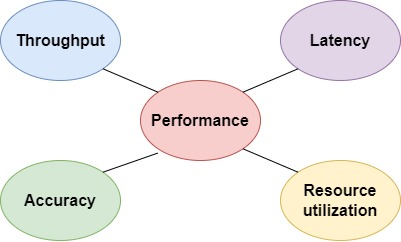
\includegraphics[width=0.6\textwidth]{pics/performance.jpg}
    \caption{Key factors for determining the performance of an AI system}
    \label{fig:performance}
\end{figure}
\\

